\documentclass[letterpaper,10pt]{article}
\usepackage[pdftex]{graphicx}
\usepackage{listings}
\usepackage{alltt}
\usepackage{color}
\usepackage{amsmath}
\usepackage{hyperref}
\usepackage{pgfplotstable}
\usepackage{float}
\usepackage[newfloat]{minted}
\usepackage{caption}
\usepackage{makeidx}

\definecolor{dkgreen}{rgb}{0,0.6,0}
\definecolor{gray}{rgb}{0.5,0.5,0.5}
\definecolor{mauve}{rgb}{0.58,0,0.82}
\definecolor{lightgray}{rgb}{.9,.9,.9}
\definecolor{darkgray}{rgb}{.4,.4,.4}
\definecolor{purple}{rgb}{0.65, 0.12, 0.82}
\definecolor{mblue}{rgb}{0,0,255}

\hypersetup{
    colorlinks,
    citecolor=black,
    filecolor=black,
    linkcolor=black,
    urlcolor=mblue
}

\makeindex

\lstset{
	basicstyle=\footnotesize,
	breaklines=true,
	 backgroundcolor=\color{white},   % choose the background color; you must add \usepackage{color} or \usepackage{xcolor}
  basicstyle=\footnotesize,        % the size of the fonts that are used for the code
  breakatwhitespace=false,         % sets if automatic breaks should only happen at whitespace
  breaklines=true,                 % sets automatic line breaking
  captionpos=b,                    % sets the caption-position to bottom
  commentstyle=\color{dkgreen},    % comment style
  deletekeywords={...},            % if you want to delete keywords from the given language
  escapeinside={\%*}{*)},          % if you want to add LaTeX within your code
  extendedchars=true,              % lets you use non-ASCII characters; for 8-bits encodings only, does not work with UTF-8
  frame=single,	                   % adds a frame around the code
  keepspaces=true,                 % keeps spaces in text, useful for keeping indentation of code (possibly needs columns=flexible)
  keywordstyle=\color{blue},       % keyword style
  otherkeywords={*,append,sub,.get,add,self,to\_list,.take,reduce\_by\_key,order\_by,flat\_map,
  ...},           % if you want to add more keywords to the set
  numbers=left,                    % where to put the line-numbers; possible values are (none, left, right)
  numbersep=5pt,                   % how far the line-numbers are from the code
  numberstyle=\tiny\color{gray}, % the style that is used for the line-numbers
  rulecolor=\color{black},         % if not set, the frame-color may be changed on line-breaks within not-black text (e.g. comments (green here))
  showspaces=false,                % show spaces everywhere adding particular underscores; it overrides 'showstringspaces'
  showstringspaces=false,          % underline spaces within strings only
  showtabs=false,                  % show tabs within strings adding particular underscores
  stepnumber=1,                    % the step between two line-numbers. If it's 1, each line will be numbered
  stringstyle=\color{mauve},     % string literal style
  tabsize=2,	                   % sets default tabsize to 2 spaces
  title=\lstname                   % show the filename of files included with \lstinputlisting; also try caption instead of title
}


\begin{document} 

\begin{titlepage}

\begin{center}

\Huge{Assignment 8}

\Large{CS532-s16:  Web Sciences}

\Large{Spring 2016}

\Large{John Berlin}

\Large Generated on \today

\end{center}

\end{titlepage}
\newpage
\printindex
\newpage
\section*{Question 1}
\index{Question 1}
\begin{verbatim}
1.  Create a blog-term matrix.  Start by grabbing 100 blogs; include:

http://f-measure.blogspot.com/
http://ws-dl.blogspot.com/

and grab 98 more as per the method shown in class.  Note that this
method randomly chooses blogs and each student will separately do
this process, so it is unlikely that these 98 blogs will be shared
among students.  In other words, no sharing of blog data.  Upload
to github your code for grabbing the blogs and provide a list of
blog URIs, both in the report and in github..

Use the blog title as the identifier for each blog (and row of the
matrix).  Use the terms from every item/title (RSS) or entry/title
(Atom) for the columns of the matrix.  The values are the frequency
of occurrence.  Essentially you are replicating the format of the
"blogdata.txt" file included with the PCI book code.  Limit the
number of terms to the most "popular" (i.e., frequent) 500 terms,
this is *after* the criteria on p. 32 (slide 7) has been satisfied.
\end{verbatim}
\subsection*{Answer}
In getting the 100 blogs and generating the blog-term matrix I wrote two python scripts
\emph{getFeeds.py} and \emph{processData.py}. The first script getFeeds.py which is seen in listing \hyperref[lst:bf]{\ref{lst:bf}} does the job of getting the blog feed data. Then processData.py seen in listing \hyperref[lst:pd]{\ref{lst:pd}} does the generation of the blog-term matrix file plus generation of following questions data.

Getting the feed data turned out to require a little bit more effort than I was expecting. The extra effort came into play when I came across blogs with no titles(blog titles). These no blog title blogs as a majority had little to no text as I found out when a great deal of my words were blanks. Also adding to the extra effort was realizing that the random next blog was not truly random rather pseudo-random as I had duplicates. Besides that the retrieval of the blog data was rather straightforward.

The blogspot API was rather straightforward and required few calls. The uris used to interact with the blogspot API can be seen on lines 12,13,14, and 15 in listing \hyperref[lst:bf]{\ref{lst:bf}}. To speed up the process of getting the feed entries I appended \emph{?max-results=200} to end of the feeds uri(\emph{feeds/posts/default}). By doing this I get a maximum of 200 entries per get request, which greatly limits the number of API calls required to get paginated entries for blogs with over 200 posts.
\newpage
I will explain the code seen in listing \hyperref[lst:bf]{\ref{lst:bf}} at first generally then break down the methods used to accomplish the task. As always consult the code seen in listing \hyperref[lst:bf]{\ref{lst:bf}} for more details in the comments.
\begin{enumerate}
\item Entire process(getData)
\begin{enumerate}
\item Check to see if the data file directory exists if not create it
\item Set up session and add user agent so we appear less like a robot
\item Consume and process the WebScience and Digital Libraries blog posts
\item Consume and process F-Measure blog posts
\item Ask for next blog 98 times, consume and process its posts
\item Write blog urls to file and write blog terms to json file called blogdata.json
\end{enumerate}
\item get98
\begin{enumerate}
\item While count is less than 98
\item Get the next blog
\item Check to see if we have already gotten it if we have choose another otherwise consume\_all
\item If what we got is nothing choose another
\item Add what we got to the data collection, increment counter by one and choose another
\end{enumerate}
\item consume\_all(start, sesh)
\begin{enumerate}
\item Ask the api for the initial set of feed entries
\item Parse the feed and get the title, if the blog has no title or if the number of entries is less than 25 choose another
\item Check to see if we have more feed entries
\item Process and flatten the initial set of feed entries
\item While we have more entries(pagination), ask for next set of feed entries, process and flatten, then check again
\item Do preliminary word count as the number of words if not reduces can cause the file size to be to big
\item Finally return the title and the blogs terms
\end{enumerate}
\item process\_text(text)
\begin{enumerate}
\item Process the feeds text using BeautifulSoup to clean out html, remove all non alpha characters then make the text lower case
\item Use nltk(natural language toolkit) to tokenize the text into words, filter the words by checking to see if they are not English language stop words
\item Return list of valid words
\end{enumerate}
\item check\_next(text)
\begin{enumerate}
\item Use BeautifulSoup to process the entire feed
\item Extract the next link(next set of feed entries) by looking for \emph{link,type: application/atom+xml, rel: next}
\item If that link exists the returned list will be of size 1, return the link and true otherwise false and none 
\end{enumerate}
\end{enumerate}

The list of 98 urls gotten can be seen in listing \hyperref[lst:uris]{\ref{lst:uris}}.

Now I will also explain the other file processData.py seen in listing \hyperref[lst:pd]{\ref{lst:pd}}, here in its entirety for the parts that go with question one. In the remain question sections I will go into detail about what was required for the parts pertaining to those remaining questions. Please note that I used \href{https://github.com/cataska/programming-collective-intelligence-code/blob/master/chapter3/clusters.py}{clusters.py} file that accompanied the book found in github repo containing the example code. 

For processing the data for the top 500 terms I created a class called feed. It allows for quick access to the preliminary word count and stem count. For another part for the next questions I stemmed the words to get a better clusters as the original method returned a very sparse term matrix leading to errors in distance calculations. Stemming the words I again used the natural language tool kit's(nltk) English stemmer to produce a correct stemming for the English language. 

The two methods in processData.py listing \hyperref[lst:pf]{\ref{lst:pd}} that partaine to question one are 
\emph{generate\_blogfile} and \emph{generate\_blogfile\_stem}. Both execute as such
\begin{enumerate}
\item generate\_blogfile
\begin{enumerate}
\item Read in the blog term json file. I use the functional python library seq class to allow for short and concise expression of the processing.
\item Get the top 500 by
\item Flattening each blogs word count
\item Filtering word count tuples for counts greater than 10(non-stemmed),1(stemmed) 
\item Do a total word count
\item Filter by the faked tfidf function
\item Sort the data in descending order 
\item Take the top 500
\item Transform the data to words only and make it a list
\item Sort the top 500 words alphabetically
\item Write the words out the blog-term matrix file
\end{enumerate}
\item generate\_blogfile\_stem
\begin{enumerate}
\item Behaves exactly like generate\_blogfile except use the stemmed word count and gets words with a count greater than 1(addendum to value used in 1d)
\end{enumerate}
\end{enumerate}

I mentioned that words with intra-document counts of 10 were used for the non-stemmed version in the explanation of 1d. Before using those values, the default count of 1 was used which lead to divide by zero exceptions in the MDS calculation. On inspection I believe it was caused by the sparse nature of the matrix terms overall. This change was done well after I had written the code for the initial implementation which lead to my usage of stemmed words. Also with this change I was able to remove my changes to the original clusters.py file which checked and poorly corrected the divide by zero exception. 
 
\newpage
\clearpage
%\inputminted[frame=single,linenos,breaklines,breakanywhere]{python3}{getFeeds.py}

\lstinputlisting[frame=single,caption={The 98 uris},label=lst:uris,captionpos=b]{datafiles/98bloguris.dat}
\clearpage
\lstinputlisting[language=Python,frame=single,
caption={Get Blog Feeds},label=lst:bf,captionpos=b]{getFeeds.py}
   
\newpage
\clearpage
\section*{Question 2}
\index{Question 2}
\begin{verbatim}
2.  Create an ASCII and JPEG dendrogram that clusters (i.e., HAC)
the most similar blogs (see slides 12 & 13).  Include the JPEG in
your report and upload the ascii file to github (it will be too
unwieldy for inclusion in the report).
\end{verbatim}
\subsection*{Answer}

The rest of the code in processData.py seen in listing \hyperref[lst:pd]{\ref{lst:pd}} deals with generating the answers to questions 2 through 4. The methods used to generate those answers are \emph{do\_non\_stem()} and \emph{do\_stemmed()}. Both operate as such:
\begin{enumerate}
\item Generate the respective blog term matrix file
\item Read the file in using the clusters.py file(from the code accompanying the programming cognitive intelligence book. 
\item Do hierarchical clustering
\item Generate text denogram and jpg denogram
\item Perform kmeans clustering and log iterations and centroid values
\item Perform dimension reduction
\item Generate dimension reduced cluster jpg
\end{enumerate}

Please note that unlike the code from the book

I included stemming as with out it we are choosing the top 500 terms out of unique 2692 terms in total.

The dendrogram generated for the nonstemmed version is seen in figure \hyperref[fig:q2deno]{\ref{fig:q2deno}} and the text version can be found in the datafiles folder file name, blogtop500\_asciideno.txt.
The dendrogram is quite large so fitting it into this report was difficult and the file name is blogtop500\_deno.jpg and is found in the datafiles directory. 

Of note the Web Science and Digital Libraries Research Group got grouped under Boggle Me Thursdays, which is under Floorshine Zipper Boots which happens to be under F-Measure. I find it interesting that the personal blog for the head of the WSDL is above the group its self.

The stemmed version is seen in figure \hyperref[fig:q2stemdeno]{\ref{fig:q2stemdeno}}. F-Measure is grouped with talk radio blogs and media blogs whereas the WSDL blog is grouped with blogs such as What am I doing(above) and The Night Mail(below). These results are more surprising to me especially for the WSDL blog.

\newpage
\begin{figure}[h]
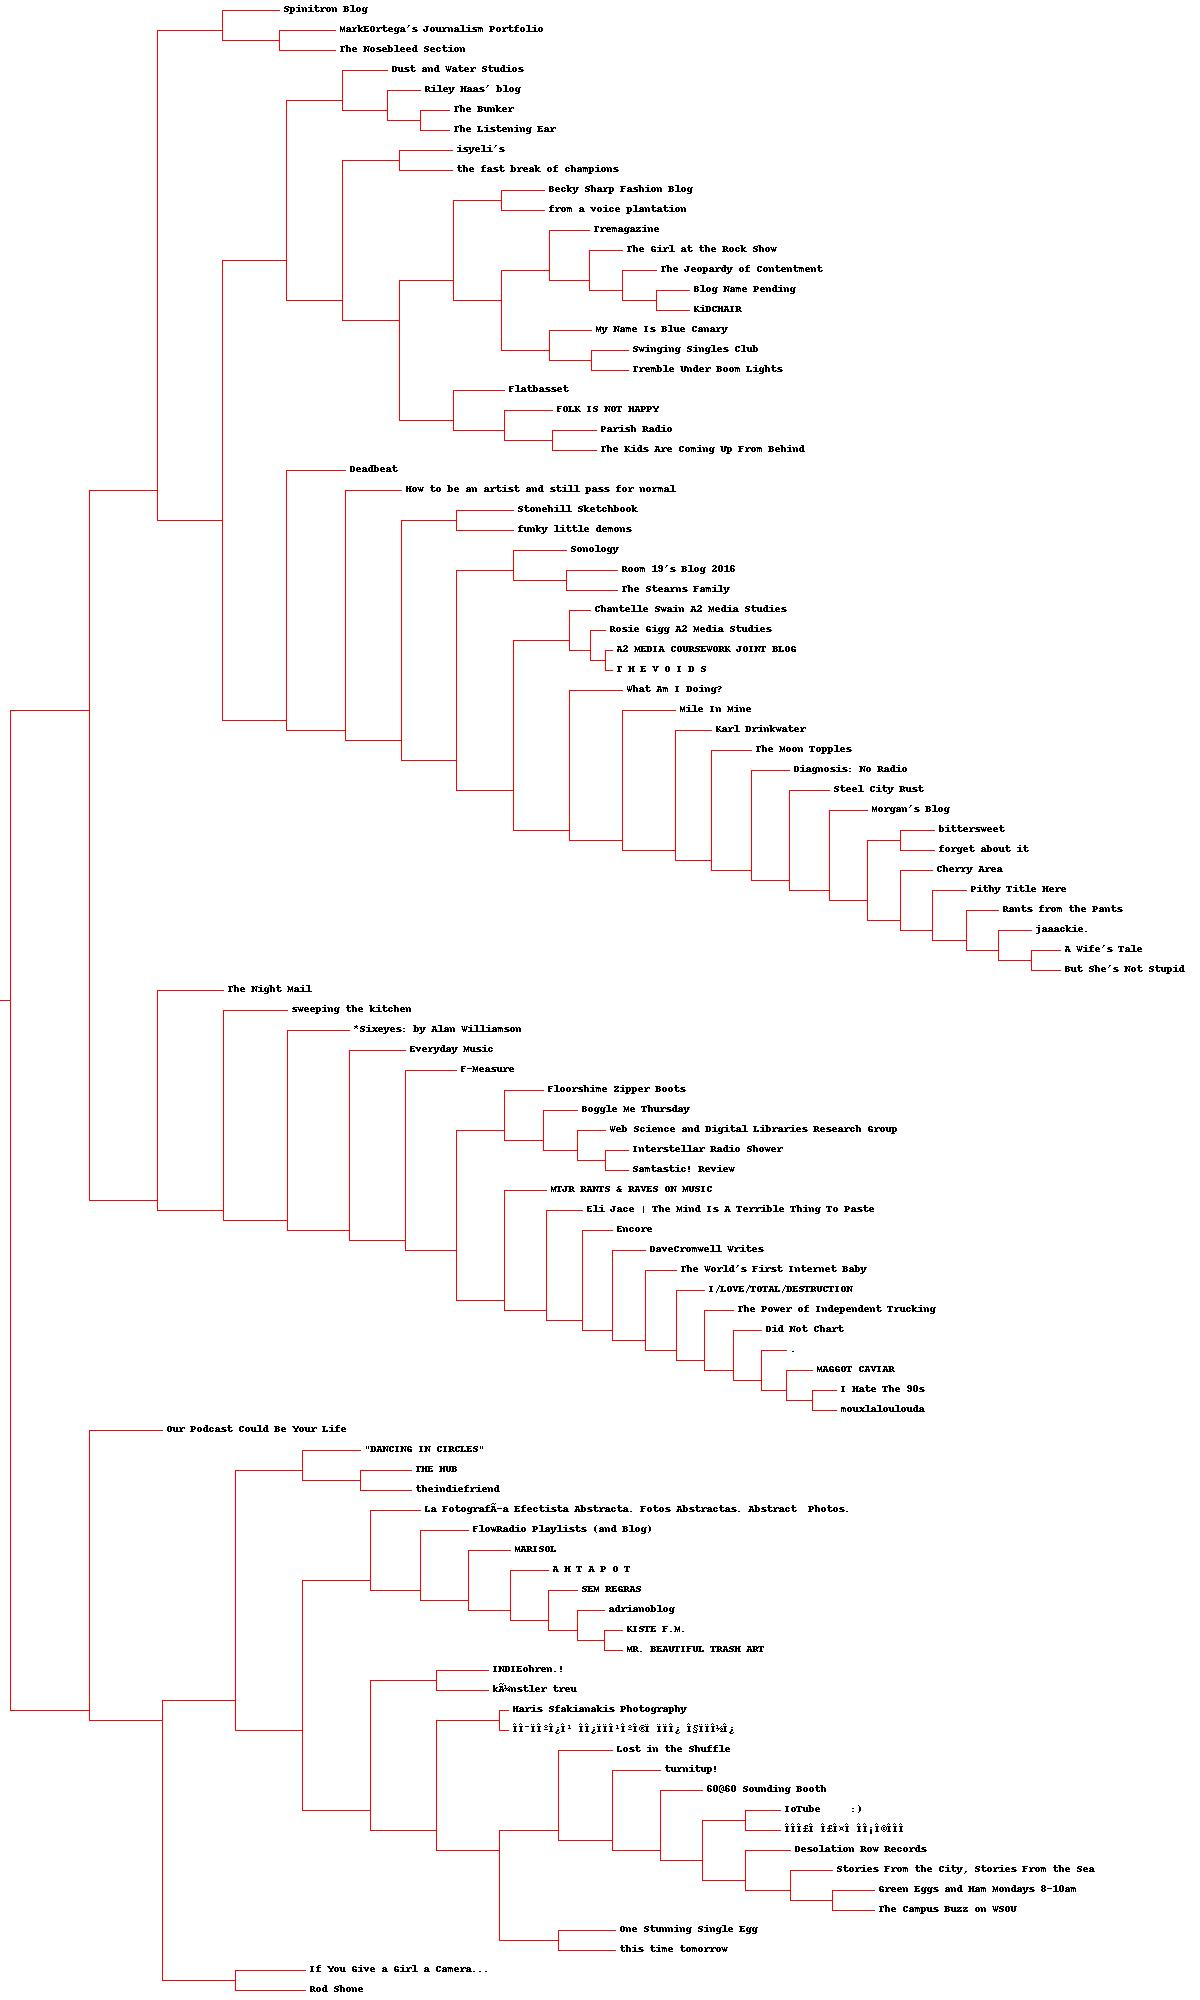
\includegraphics[scale=0.26]{datafiles/blogtop500_deno.jpg}
\caption{Dendogram of the blogs using top 500 terms}
\label{fig:q2deno}
\end{figure}
\newpage
\begin{figure}[h]
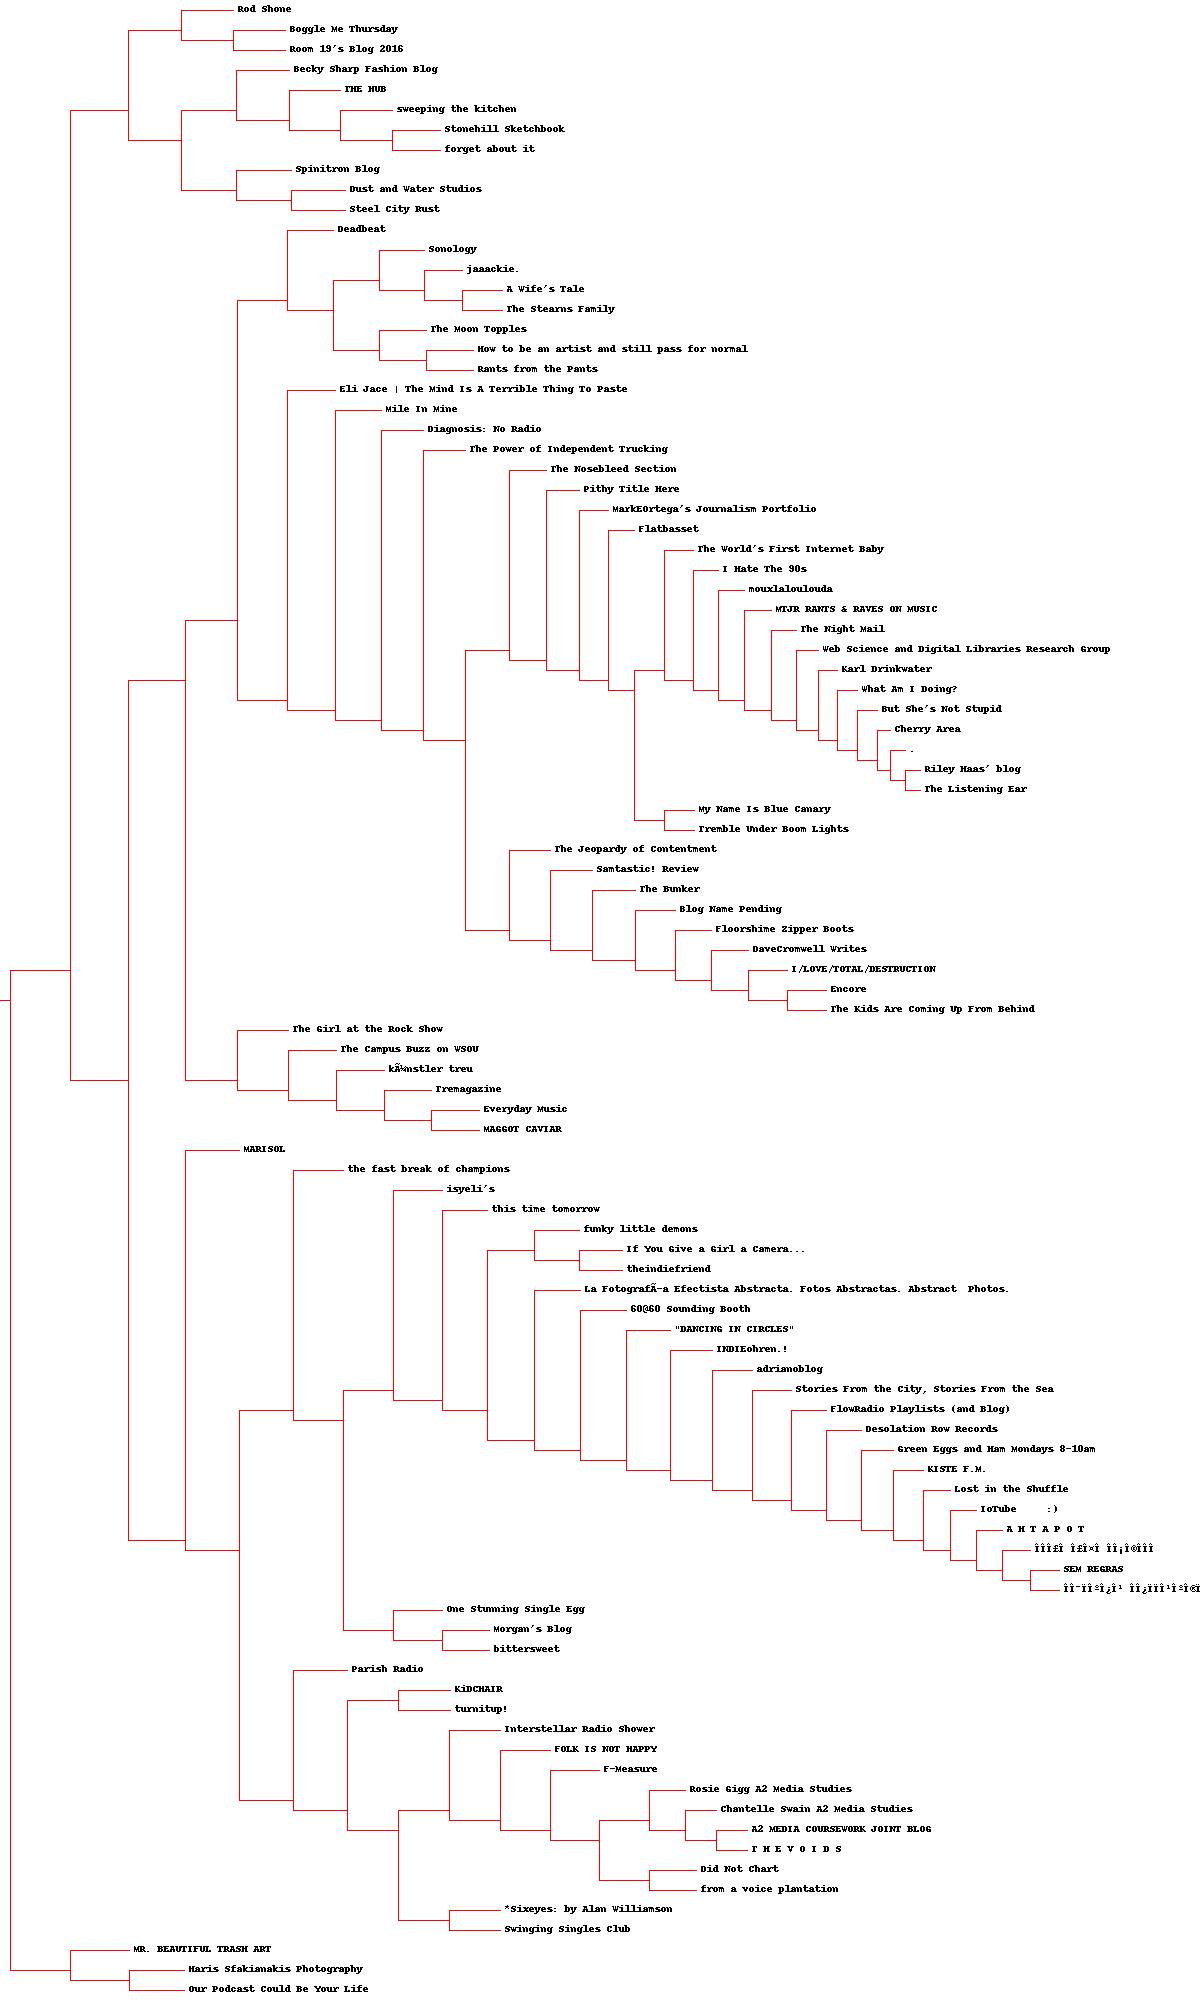
\includegraphics[scale=0.26]{datafiles/blogtop500stemmed_deno.jpg}
\caption{Dendogram of the blogs using top 500 stemmed terms}
\label{fig:q2stemdeno}
\end{figure}
\newpage
\lstinputlisting[language=Python,frame=single,
caption={Process Feed Data and Generate Output},label=lst:pd,captionpos=b]{processData.py}   

\section*{Question 3}
\index{Question 3}
\begin{verbatim}
3.  Cluster the blogs using K-Means, using k=5,10,20. (see slide
18).  Print the values in each centroid, for each value of k.  How
many interations were required for each value of k?
\end{verbatim}
\subsection*{Answer}
The full output of kmeans can be seen in listing \hyperref[lst:kmeans]{\ref{lst:kmeans}} for non-stemmed and \hyperref[lst:kmeansstem]{\ref{lst:kmeansstem}} for stemmed. For non-stemmed k=5 took 8 iterations, k=10 took 4, and k=20 took 4 as well. The stemmed version for k=5 took 6 iterations, k=10 took 5 and k=20 took 3.

\newpage
\lstinputlisting[frame=single,caption={Kmeans output non-stemmed},label=lst:kmeans,captionpos=b]{datafiles/kmeans_blogtop500.txt}
\lstinputlisting[frame=single,caption={Kmeans output stemmed},label=lst:kmeansstem,captionpos=b]{datafiles/kmeans_blogtop500stemmed.txt}
\newpage
\section*{Question 4}
\index{Question 4}
\begin{verbatim}
4.  Use MDS to create a JPEG of the blogs similar to slide 29.  
How many iterations were required?
\end{verbatim}
\subsection*{Answer}
The number of iterations required for dimension reduction for both the non-stemmed and stemmed versions can bee seen below in listings \hyperref[lst:drns]{\ref{lst:drns}} and \hyperref[lst:drs]{\ref{lst:drs}}.
\lstinputlisting[frame=single,caption={Dimension Reduction Iterations Non-Stemmed},label=lst:drns,captionpos=b]{datafiles/dimensionReductionNonStemmed.txt}
\lstinputlisting[frame=single,caption={Dimension Reduction Iterations Stemmed},label=lst:drs,captionpos=b]{datafiles/dimensionReductionStemmed.txt}

The difference in the number of iterations for the dimension reduction between the non-stemmeed and stemmed blog term matrices in my opion is due to the sparse nature of the terms. The raw terms are very different as the blogs gotten are all over the place in terms of content thus it will take longer. Whereas the stemmed version the context of the words is removed and a better approximation can be made. 

The resultant jpg pictures can be seen in figure \hyperref[fig:dim]{\ref{fig:dim}} for non-stemmed and \hyperref[fig:dimstem]{\ref{fig:dimstem}} for stemmed. Once again these pictures are way to large to clearly see in this report. For clearer inspect the files are found in datafiles/blogtop500\_clust2d.jpg and datafiles/blogtop500stemmed\_clust2d.jpg. 

Of note in blogtop500\_clust2d.jpg, the WSDL blog is grouped with Stories From the City, Stories from the Sea and F-Measure is grouped with The Kids are Coming Up From Behind.

Also of note in blogtop500stemmed\_clust2d.jpg, the WSDL blog is grouped with The Night Mail and F-Measure is grouped with MarkEOrtega's Journalism Portfolio.

\newpage
\begin{figure}[htbp]
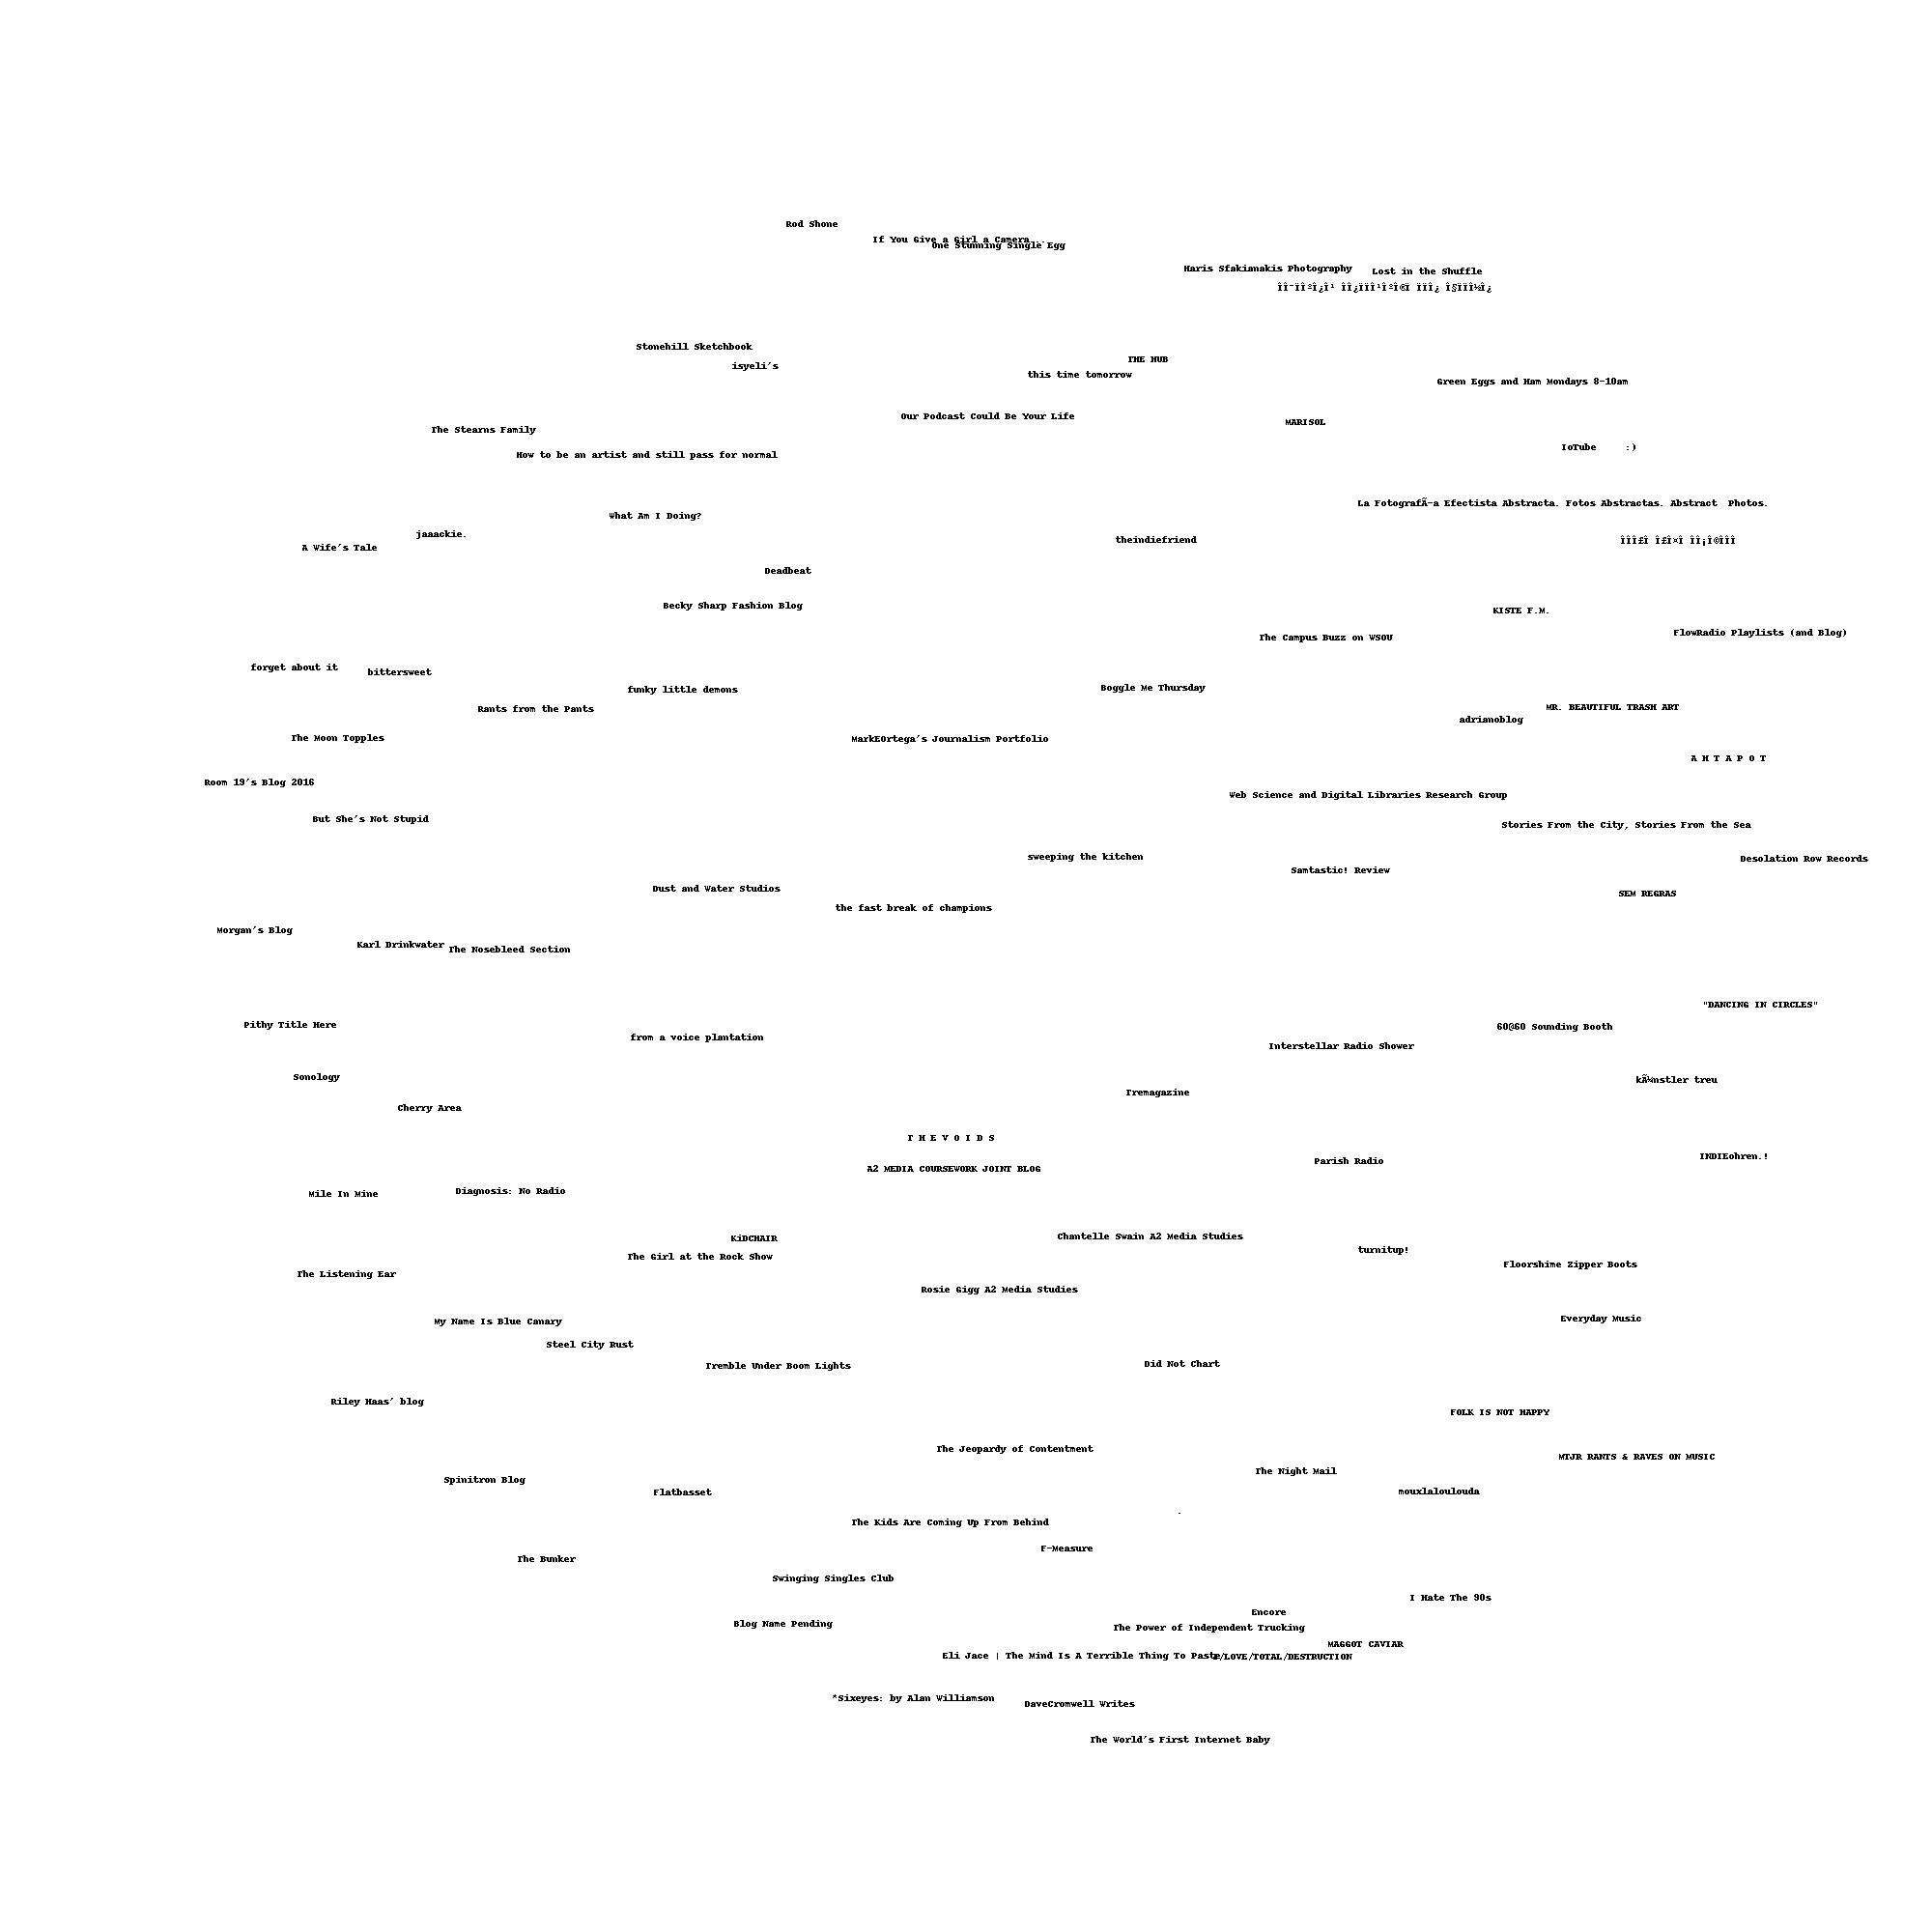
\includegraphics[scale=0.20]{datafiles/blogtop500_clust2d.jpg}
\caption{Dimension Reduction Non Stemmed}
\label{fig:dim}
\end{figure}
\newpage
\begin{figure}[htbp]
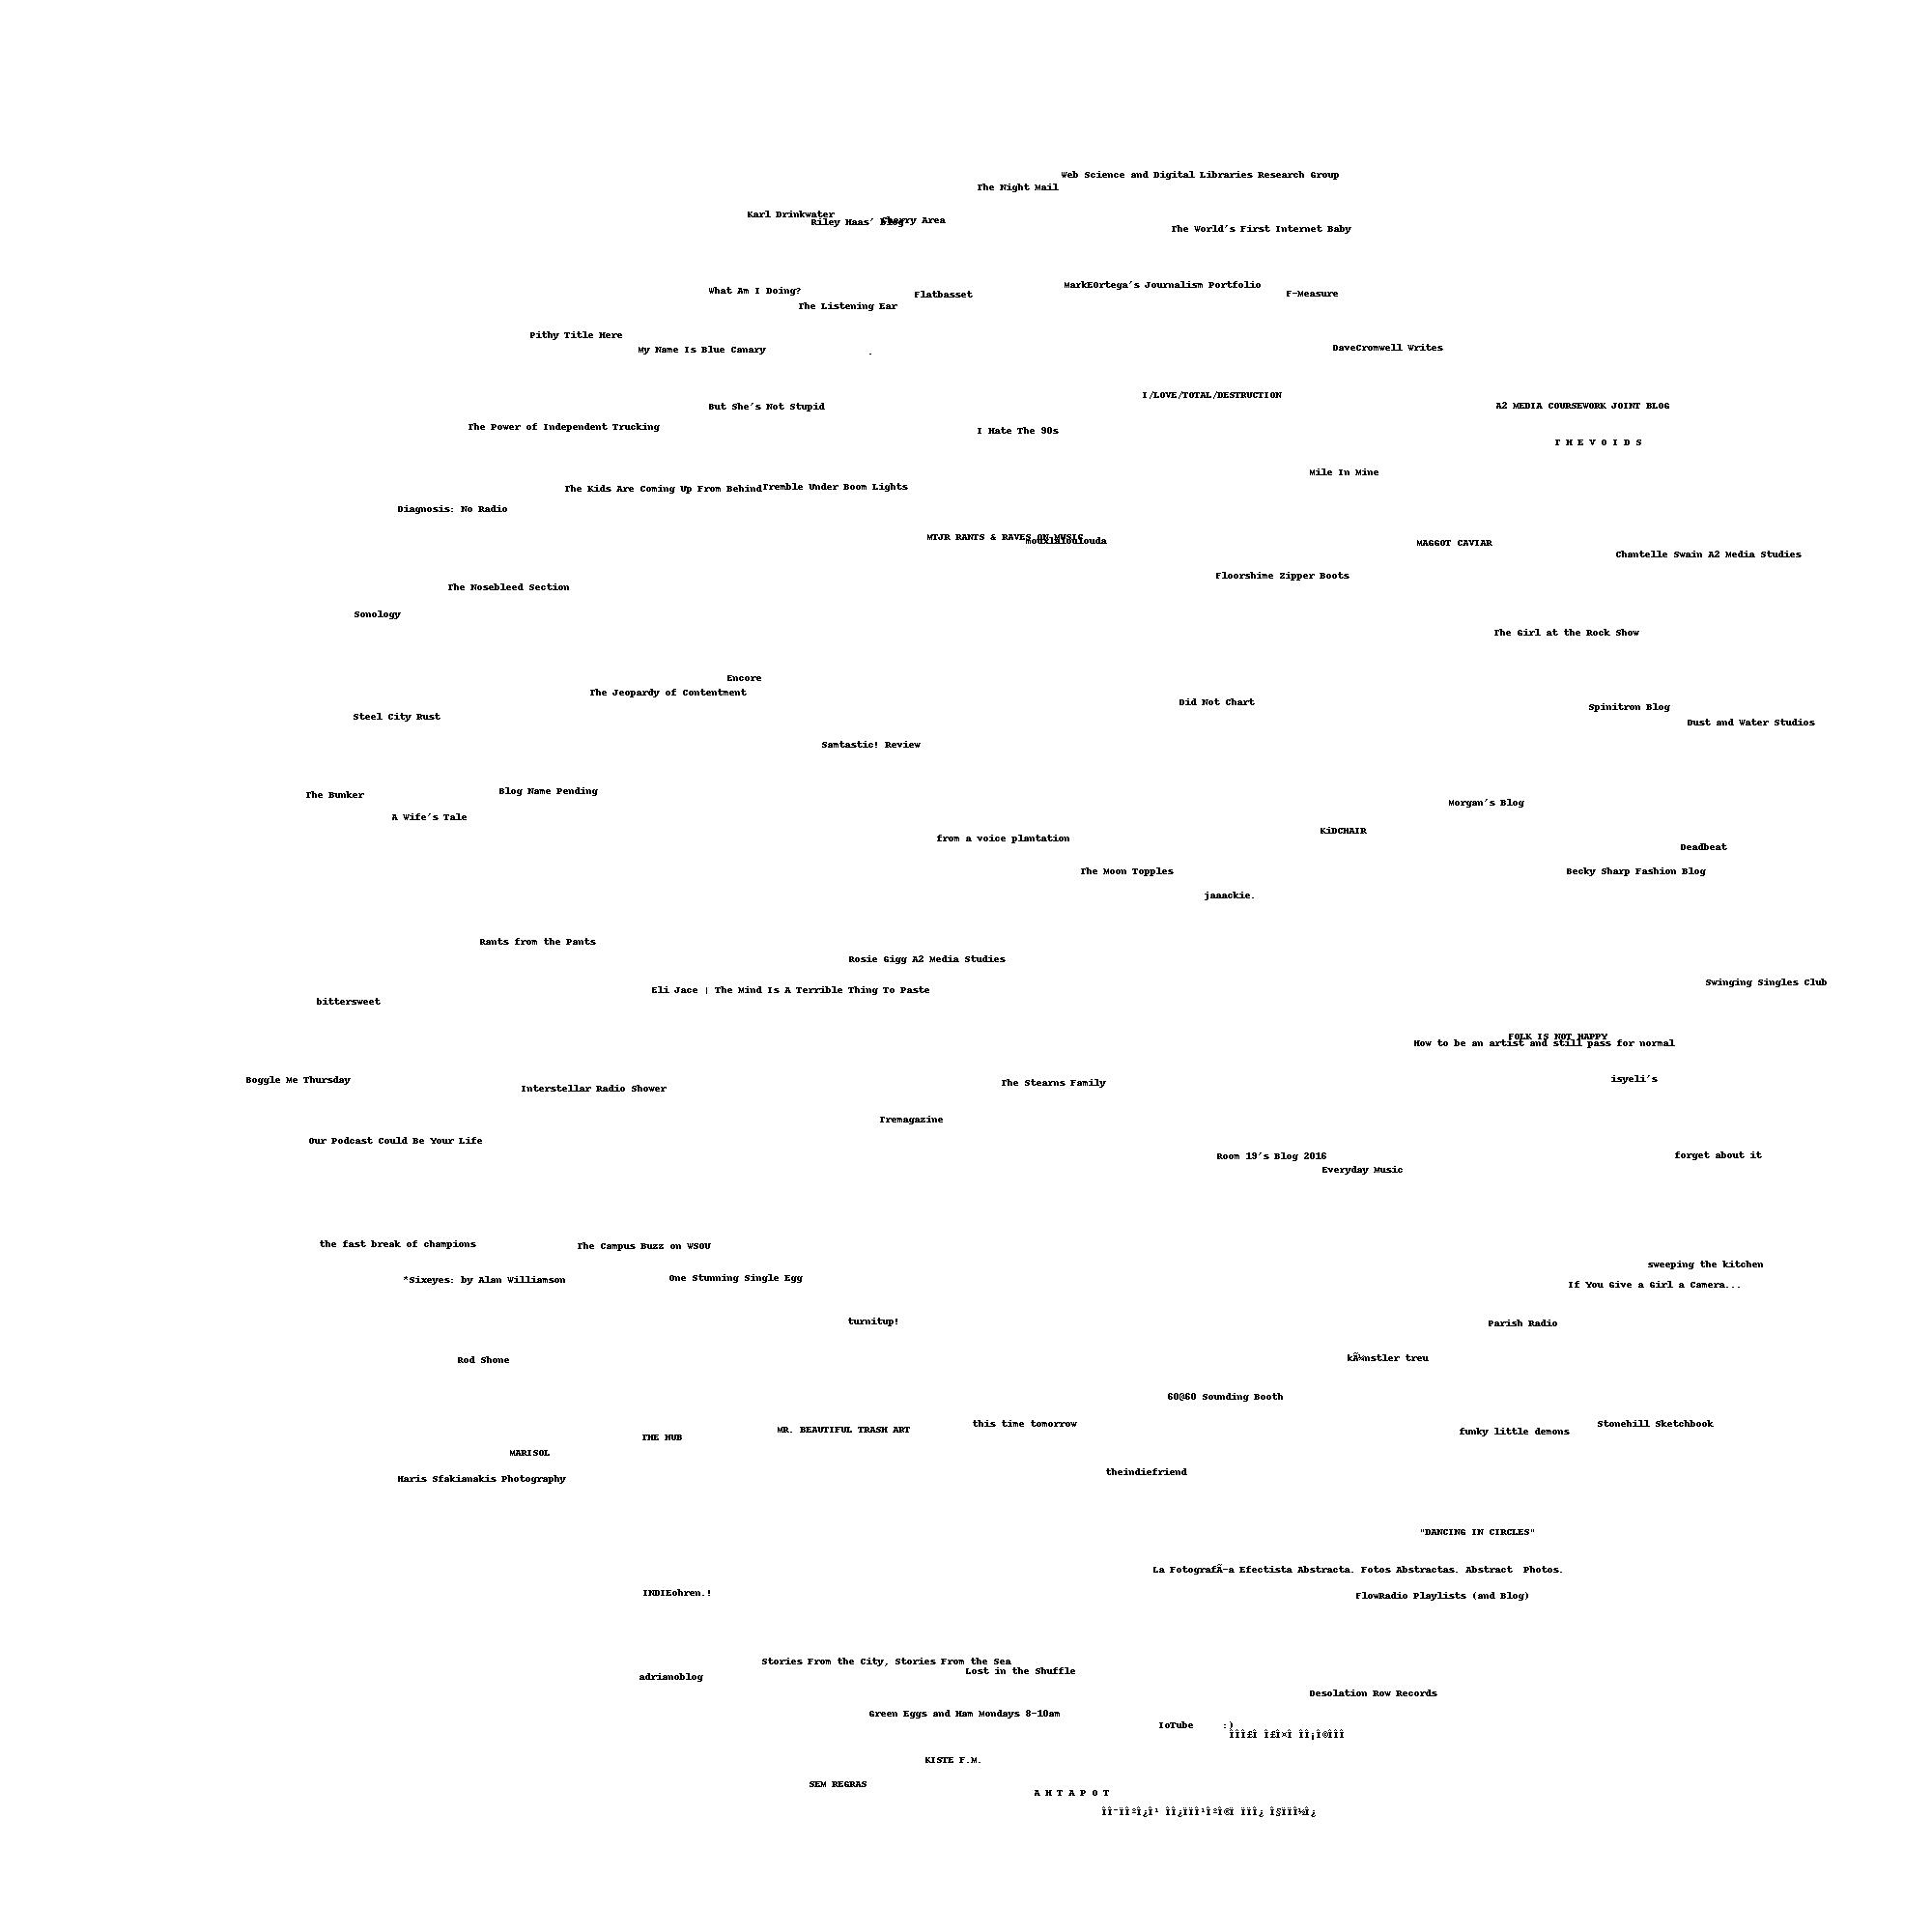
\includegraphics[scale=0.20]{datafiles/blogtop500stemmed_clust2d.jpg}
\caption{Dimension Reduction Stemmed}
\label{fig:dimstem}
\end{figure}
\newpage
\section*{Question 5}
\index{Question 5}
\begin{verbatim}
5.  Re-run question 2, but this time with proper TFIDF calculations
instead of the hack discussed on slide 7 (p. 32).  Use the same 500
words, but this time replace their frequency count with TFIDF scores
as computed in assignment #3.  Document the code, techniques,
methods, etc. used to generate these TFIDF values.  Upload the new
data file to github.

Compare and contrast the resulting dendrogram with the dendrogram
from question #2.

Note: ideally you would not reuse the same 500 terms and instead
come up with TFIDF scores for all the terms and then choose the top
500 from that list, but I'm trying to limit the amount of work
necessary.
w many iterations were required?

===================================================================
========The questions below is for 5 points extra credit===========
===================================================================
\end{verbatim}
\subsection*{Answer}
Not attempted. 
\end{document}